% Frame 1: Algorithms
\begin{frame}
    \frametitle{Different Algorithms}
    We implement the following algorithms throughout our assignments:
    \begin{itemize}
        \item K-Nearest Neighbors
        \item Nearest Centroid
        \item Convolutional Neural Network (CNN)
        \item Multi-Layer Perceptron (MLP)
        \item Support Vector Machine (SVM)
        \item Transformer
    \end{itemize}
    We will compare them with each other while explaining the way they work. We will also 
    be mentioning some \textbf{extra} things we tried.
\end{frame}

% Frame 2: Dataset
\begin{frame}
    \frametitle{Dataset}
    For the first two assignments we chose to go with CIFAR-10. A dataset which sports:
    \begin{itemize}
        \item 60,000 32x32 color images
        \item 10 classes, with 6,000 images per class
        \item 50,000 training images 
        \item 10,000 test images
    \end{itemize}
    The simplest algorithms we tried training the dataset on were K-Nearest Neighbors and 
    Nearest Centroid. Let's see them in greater detail.
\end{frame}

% Frame 3: CIFAR-10 Visualization
\begin{frame}
    \frametitle{CIFAR-10 Visualization}
    \begin{figure}
        \centering
        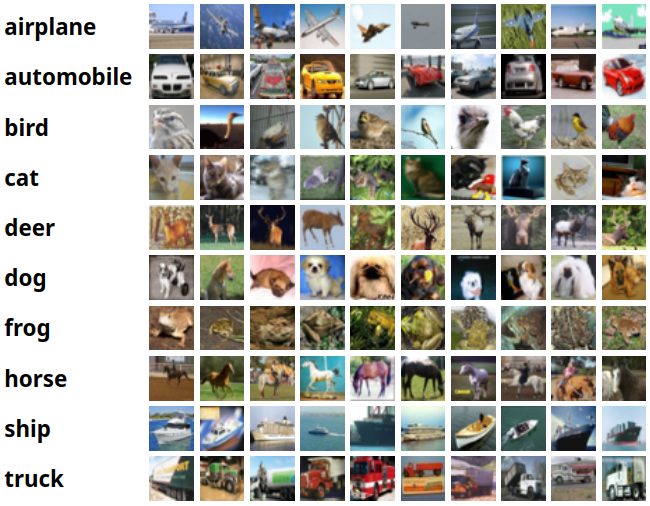
\includegraphics[width=0.6\textwidth]{media/1stAssignment/cifar10_example.png}
        \caption{CIFAR-10 Dataset}
    \end{figure}
\end{frame}

% Frame 4: K-Nearest Neighbor
\begin{frame}
\frametitle{K Nearest Neighbor}
\begin{center}
    How does it work?
\end{center}
\begin{columns}
    \begin{column}{0.5\textwidth}
        We calculate the distance between each point in the test dataset with all the point from
        the training dataset. We then select the k-nearest points and classify the test point.
    \end{column}

    \begin{column}{0.45\textwidth}
        \begin{figure}
            \centering
            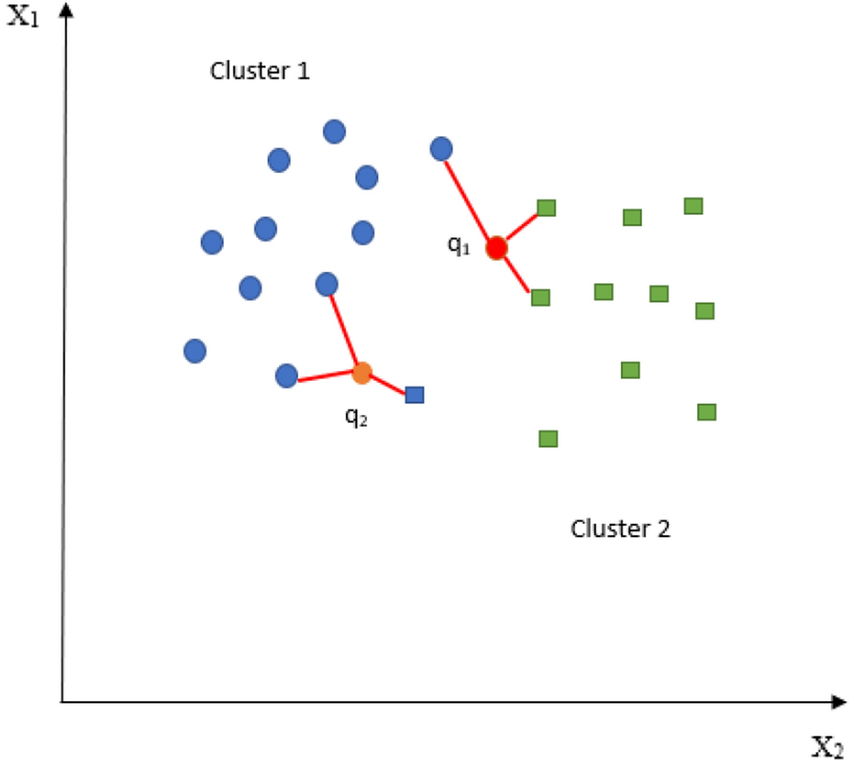
\includegraphics[width=1\textwidth]{media/1stAssignment/knn_example.png}
            \caption{K-Nearest Neighbors}
        \end{figure}
    \end{column}
\end{columns}
\end{frame}

% Frame 5: Nearest Centroid
\begin{frame}
\frametitle{Nearest Centroid}
\begin{center}
    How does it work?
\end{center}

\begin{columns}
    \begin{column}{0.5\textwidth}
        We calculate the centroid of each class in the training dataset and then compare the 
        distance of the test point with each centroid. We classify the test point to the class
        with the closest centroid.
    \end{column}

    \begin{column}{0.5\textwidth}
        \begin{figure}
            \centering
            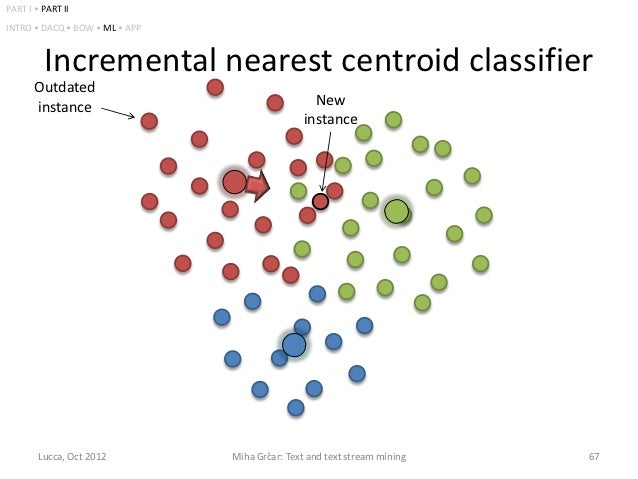
\includegraphics[width=1\textwidth]{media/1stAssignment/centroid_example.jpg}
            \caption{Nearest Centroid}
        \end{figure}
    \end{column}
\end{columns}
\end{frame}

% Frame 6: K-Nearest Neighbor vs Nearest Centroid
\begin{frame}
\frametitle{K-Nearest Neighbor vs Nearest Centroid}
\begin{figure}[H]
    \centering
    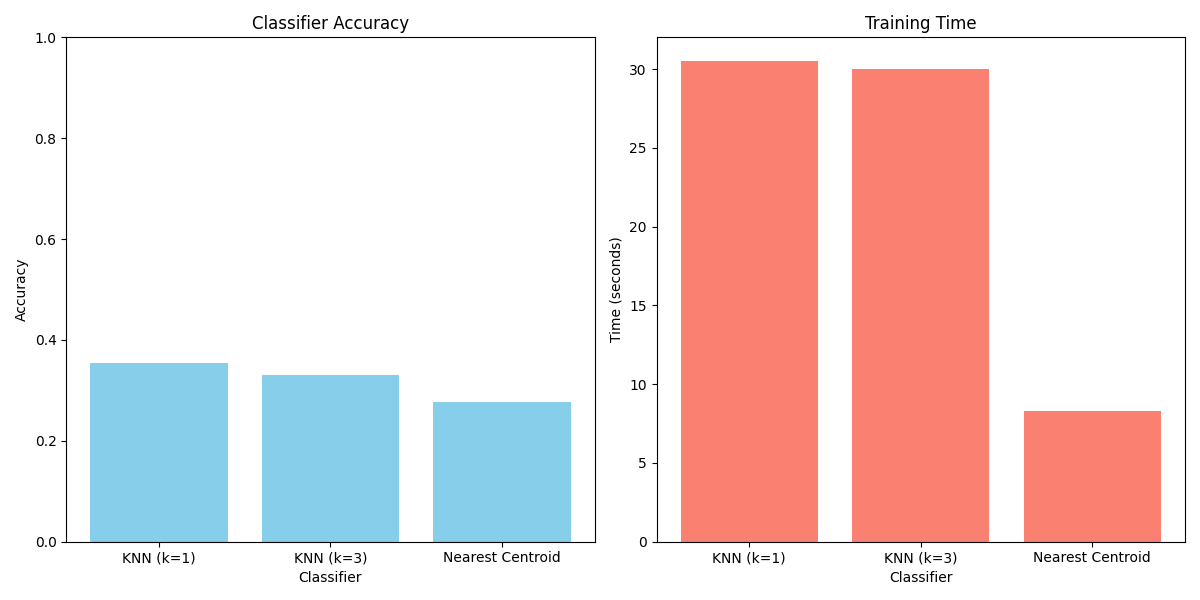
\includegraphics[width=1\textwidth]{media/2ndAssignment/knn_centroid.png}
    \caption{K-Nearest Neighbor vs Nearest Centroid}
\end{figure}
\end{frame}

% Frame 7: Speed and Performance
\begin{frame}
\frametitle{Speed and Performance}
\center \textbf{Speed}
\begin{itemize}
    \item \textbf{K-Nearest Neighbor:} Distance calculation of every test point with each training point.
    \item \textbf{Nearest Centroid:} Distance calculation of every test point with each centroid.
\end{itemize}
\center \textbf{Performance}\\
Very similar performance between the two.
\end{frame}

% Frame 8: Convolutional Neural Network
\begin{frame}
\frametitle{Convolutional Neural Network}
It is the first complex algorithm we tried. Here are the network characteristics we stuck to:
\begin{columns}
    \begin{column}{0.5\textwidth}
        \begin{itemize}
            \item 6 Convolutional Layers
            \item 3 Max Pooling Layers $2 \times 2$ with Dropout $0.25$
            \item 2 Fully Connected Layers with Dropout $0.5$
            \item 1 Output Layer
            \item ReLU Activation Function
            \item Adam Optimizer
            \item Cross Entropy Loss
            \item Reduce Learning Rate on Plateau
        \end{itemize}
    \end{column}
    \begin{column}{0.5\textwidth}
        \begin{itemize}
            \item Dataset transformations such as:
            \begin{itemize}
                \item Random Horizontal Flip
                \item Random Rotation
                \item Random Crop    
            \end{itemize}
            \item Normalization around 0.5 for the mean and 0.2 for the standard deviation
        \end{itemize}
    \end{column}
\end{columns}
\end{frame}

% Frame 9: Learning Rate Scheduler
\begin{frame}
\frametitle{Reduce Learning Rate on Plateau}
\center How does it work?
\begin{itemize}
    \item We monitor the test loss
    \item Reduces LR after 3 epochs of no improvement
    \item When it does reduce, it does so by a factor of 0.5
\end{itemize}
\end{frame}

% Frame 10: Manual Testing Script
\begin{frame}
\frametitle{Manual Testing Script}
\begin{columns}[t]
    \begin{column}{0.5\textwidth}    
        Custom script aiming to test performance on non-CIFAR-10 images.\\
        Options include testing on:
        \begin{itemize}
            \item A Random Image
            \item A Random CIFAR-10 Image
            \item A Batch of Random Images
        \end{itemize}
        On the right we can see an example output of the script.
    \end{column}

    \begin{column}{0.5\textwidth}
        \begin{figure}
            \centering
            \vspace{-1cm}
            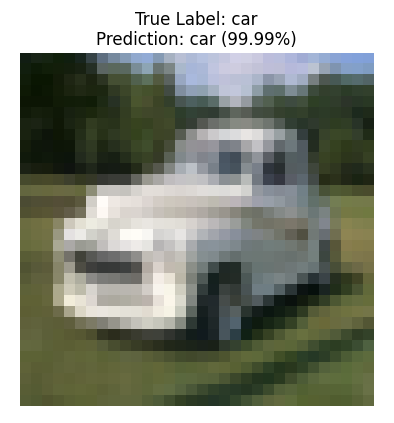
\includegraphics[width=0.9\textwidth]{media/1stAssignment/random_cifar.png}
            \vspace{-0.3cm}
            \caption{A Random CIFAR-10 Image: Example Output}
        \end{figure}
    \end{column}
\end{columns}
\end{frame}

% Frame 11: Additional Testing Example
\begin{frame}
    \frametitle{Additional Testing Example}
    \vspace{-0.25cm}
    \begin{figure}
        \centering
        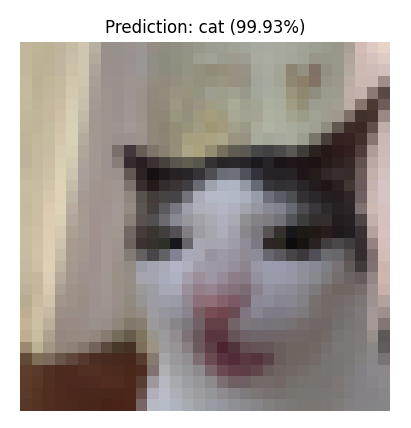
\includegraphics[height=0.7\textheight]{media/1stAssignment/custom_image.png}
        \vspace{-0.3cm}
        \caption{A Random Image: Example Output}
    \end{figure}
    \vspace{-0.4cm}
    \center \small Label is embedded in the filename and used to cross-reference the prediction.
\end{frame}

% Frame 12: Manual Testing Results
\begin{frame}
\frametitle{Manual Testing Results}
\begin{columns}
    \begin{column}{0.5\textwidth}
        \begin{figure}
            \centering
            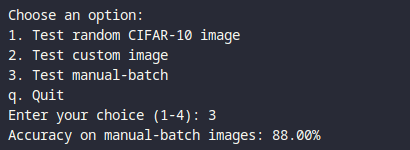
\includegraphics[width=1\textwidth]{media/1stAssignment/manual_batch.png}
            \caption{Manual Testing Results}
        \end{figure}
    \end{column}

    \begin{column}{0.5\textwidth}
        Observations:
        \begin{itemize}
            \item Slightly worse performance 
            \item Not much over-fitting
        \end{itemize}
    \end{column}
\end{columns}
\end{frame}

% Frame 13: Modifications
\begin{frame}
\frametitle{Modifications}
We tried changing the following parameters:
\begin{itemize}
    \item Activation Function
    \item Optimizer
    \item Normalization values
    \item Architecture
\end{itemize}
\end{frame}

% Frame 14: Activation Function modifications
\begin{frame}
\frametitle{Activation Function: ReLU vs Tanh}
\begin{columns}
    \begin{column}{0.5\textwidth}
        \begin{figure}[t]
            \centering
            \vspace{-0.4cm}
            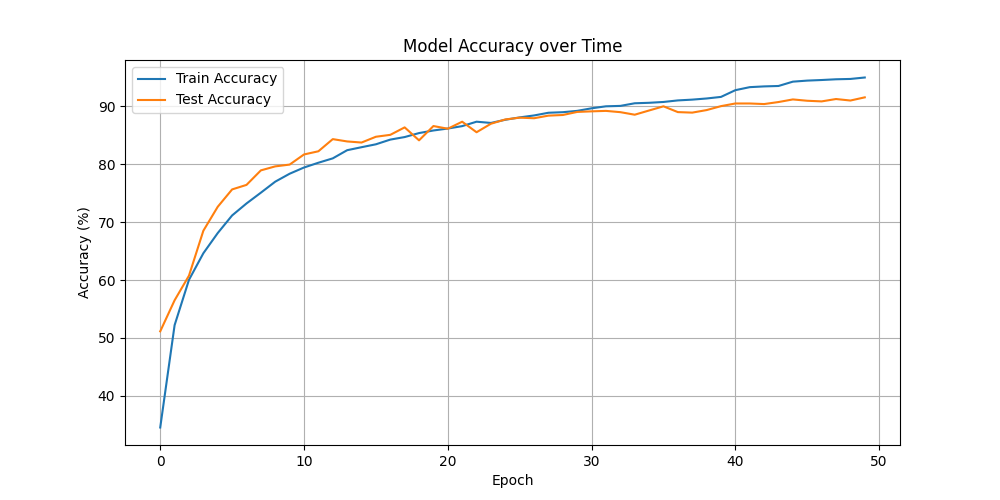
\includegraphics[width=0.9\textwidth]{media/1stAssignment/cifar10_cnn_accuracy.png}
        \end{figure}
        \vspace{-0.8cm}
        \begin{figure}[t]
            \centering
            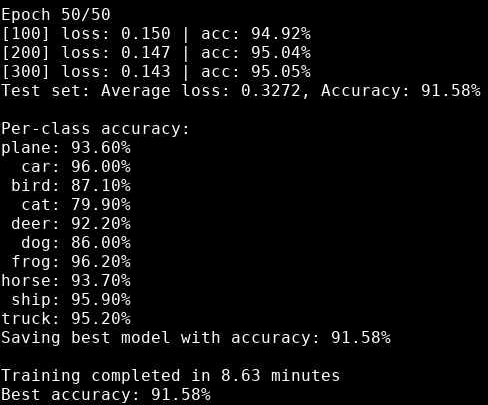
\includegraphics[width=0.9\textwidth]{media/1stAssignment/cnn_epoch_50.png}
            \vspace{-0.3cm}
            \caption{ReLU: Last Epoch}
        \end{figure}
    \end{column}

    \begin{column}{0.5\textwidth}
        \begin{figure}[t]
            \centering
            \vspace{-0.4cm}
            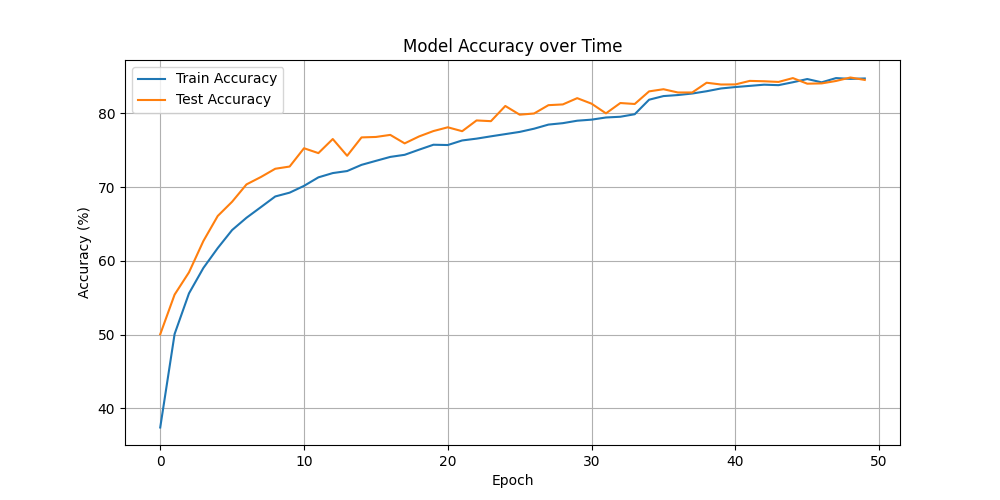
\includegraphics[width=0.9\textwidth]{media/1stAssignment/cifar10_cnn_tanh_accuracy.png}
        \end{figure}
        \vspace{-0.8cm}
        \begin{figure}[t]
            \centering
            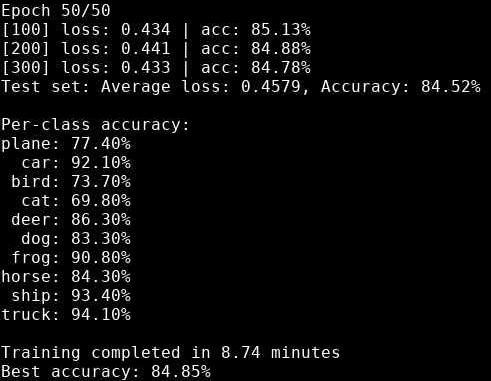
\includegraphics[width=0.9\textwidth]{media/1stAssignment/cnn_tanh_epoch_50.png}
            \vspace{-0.3cm}
            \caption{Tanh: Last Epoch}
        \end{figure}
    \end{column}    
\end{columns}
\end{frame}

% Frame 15: Optimizer modifications
\begin{frame}
\frametitle{Optimizer: Adam vs SGD}
\begin{columns}
    \begin{column}{0.5\textwidth}
        \begin{figure}[t]
            \centering
            \vspace{-0.4cm}
            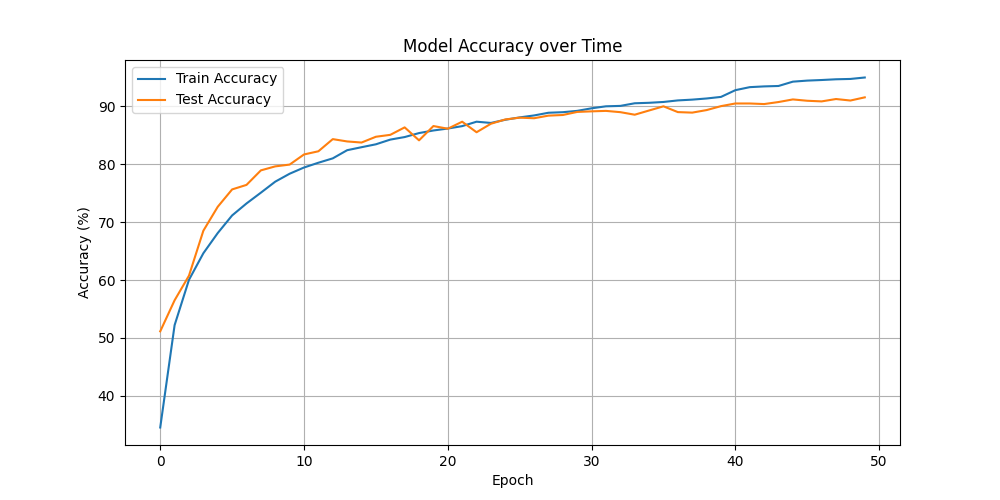
\includegraphics[width=0.9\textwidth]{media/1stAssignment/cifar10_cnn_accuracy.png}
        \end{figure}
        \vspace{-0.8cm}
        \begin{figure}[t]
            \centering
            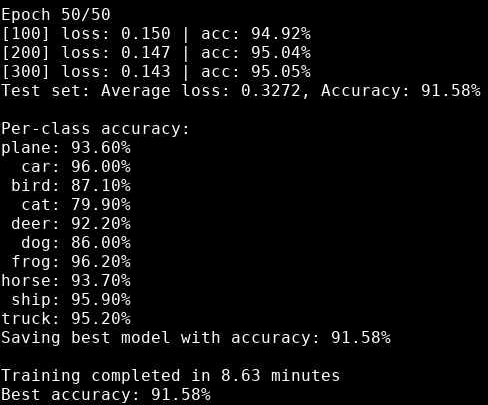
\includegraphics[width=0.9\textwidth]{media/1stAssignment/cnn_epoch_50.png}
            \vspace{-0.3cm}
            \caption{Adam: Last Epoch}
        \end{figure}
    \end{column}

    \begin{column}{0.5\textwidth}
        \begin{figure}[t]
            \centering
            \vspace{-0.4cm}
            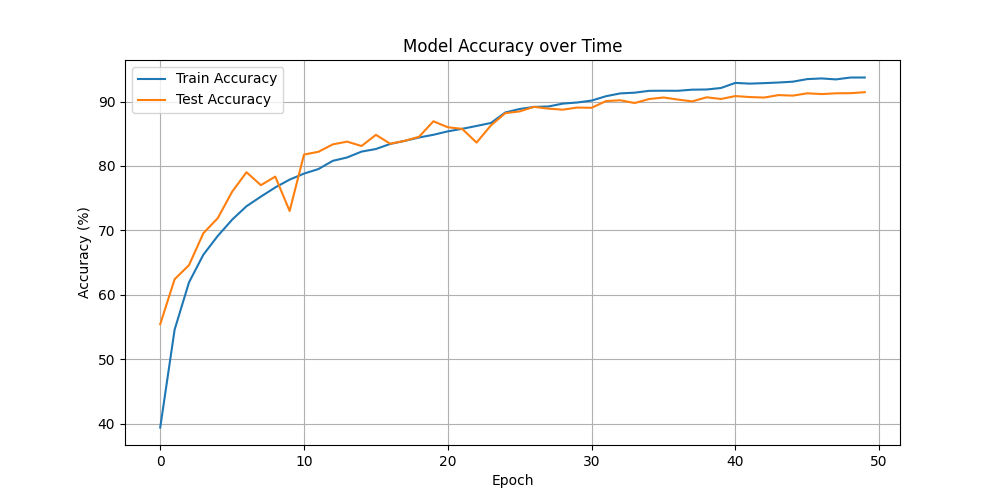
\includegraphics[width=0.9\textwidth]{media/1stAssignment/cifar10_cnn_sgd_accuracy.png}
        \end{figure}
        \vspace{-0.8cm}
        \begin{figure}[t]
            \centering
            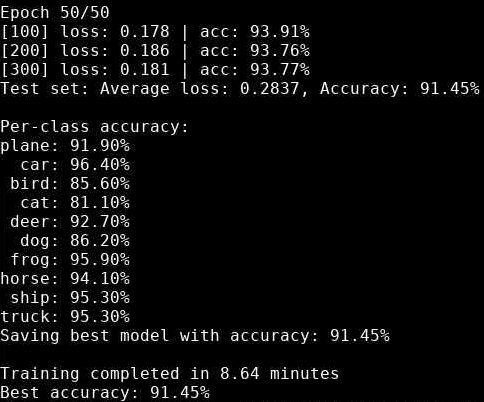
\includegraphics[width=0.9\textwidth]{media/1stAssignment/cnn_sgd_epoch_50.png}
            \vspace{-0.3cm}
            \caption{SGD: Last Epoch}
        \end{figure}
    \end{column}
\end{columns}
\end{frame}

% Frame 16: Normalization modifications
\begin{frame}
\frametitle{Normalization value Variations}
\begin{columns}
    \begin{column}{0.4\textwidth}
        \vspace{-0.1cm}
        \begin{figure}[t]
            \centering
            \vspace{-0.4cm}
            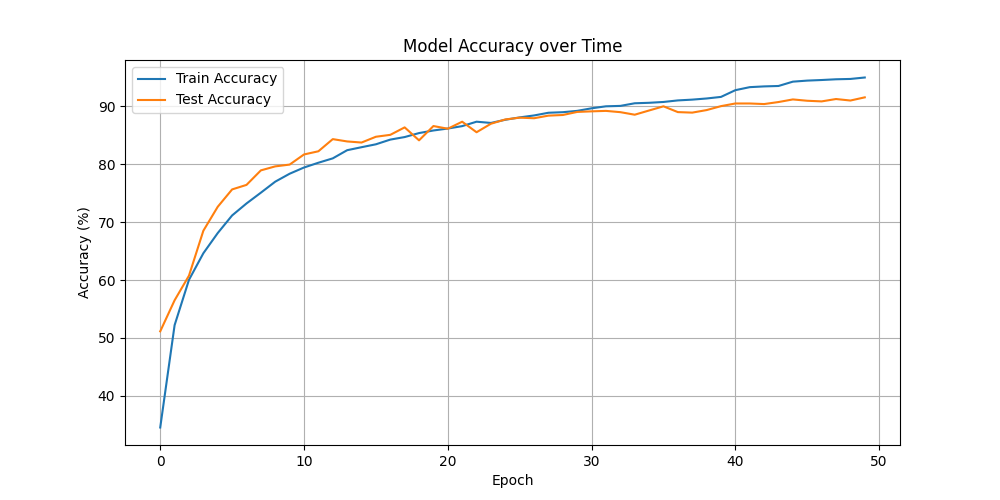
\includegraphics[width=0.9\textwidth]{media/1stAssignment/cifar10_cnn_accuracy.png}
        \end{figure}
        \vspace{-0.6cm}
        \begin{figure}[t]
            \centering
            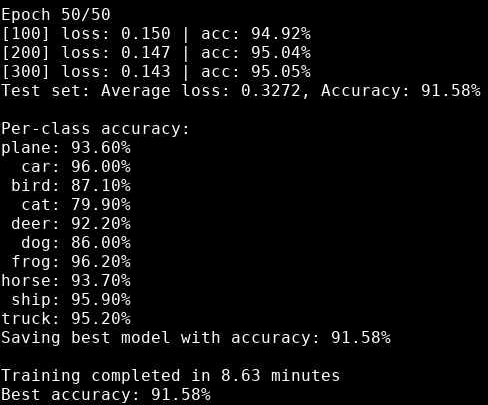
\includegraphics[width=0.9\textwidth]{media/1stAssignment/cnn_epoch_50.png}
            \vspace{-0.3cm}
            \caption{Optimized}
        \end{figure}
        \vspace{-0.6cm}
        \center \tiny Mean: (0.4914, 0.4822, 0.4465),
        \vspace{-0.3cm}
        \center \tiny Standard Deviation: (0.2023, 0.1994, 0.2010)
    \end{column}

    \begin{column}{0.4\textwidth}
        \vspace{-0.1cm}
        \begin{figure}[t]
            \centering
            \vspace{-0.4cm}
            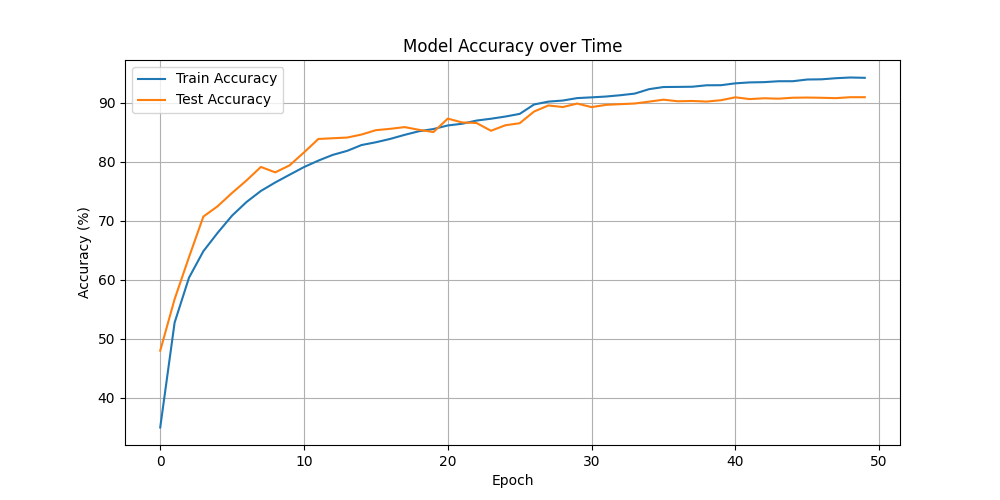
\includegraphics[width=0.9\textwidth]{media/1stAssignment/cifar10_cnn_std_accuracy.png}
        \end{figure}
        \vspace{-0.6cm}
        \begin{figure}[t]
            \centering
            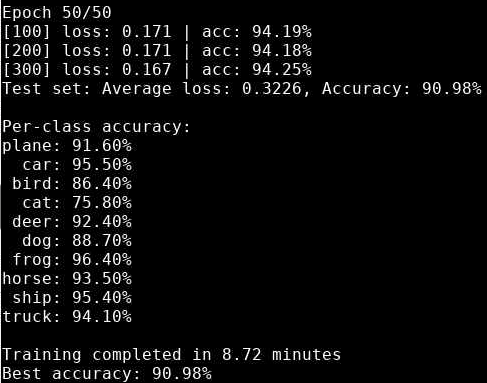
\includegraphics[width=0.9\textwidth]{media/1stAssignment/cnn_std_epoch_50.png}
            \vspace{-0.3cm}
            \caption{Standard}
        \end{figure}
        \vspace{-0.6cm}
        \center \tiny Mean: (0.5, 0.5, 0.5),
        \vspace{-0.3cm}
        \center \tiny Standard Deviation: (0.5, 0.5, 0.5)
    \end{column}

    \begin{column}{0.4\textwidth}
        \vspace{-0.1cm}
        \begin{figure}[t]
            \centering
            \vspace{-0.4cm}
            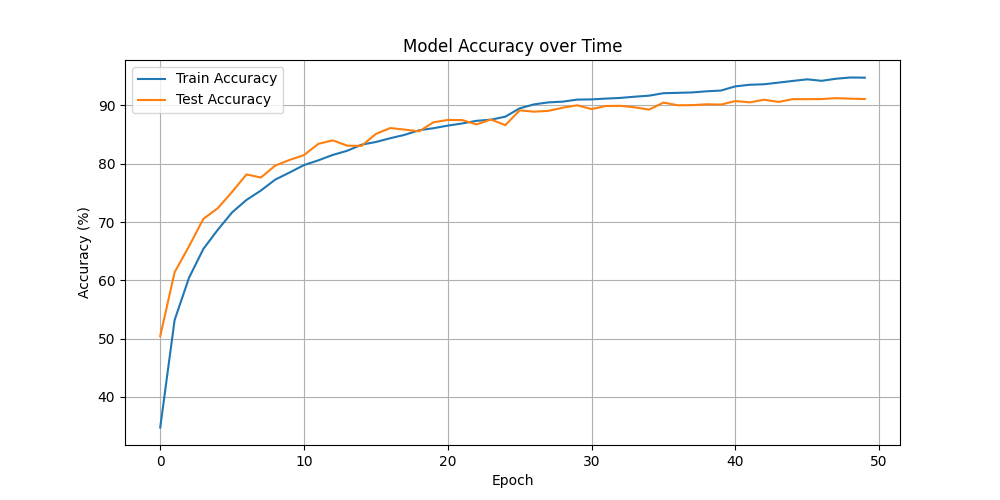
\includegraphics[width=0.9\textwidth]{media/1stAssignment/cifar10_cnn_zero_accuracy.png}
        \end{figure}
        \vspace{-0.6cm}
        \begin{figure}[t]
            \centering
            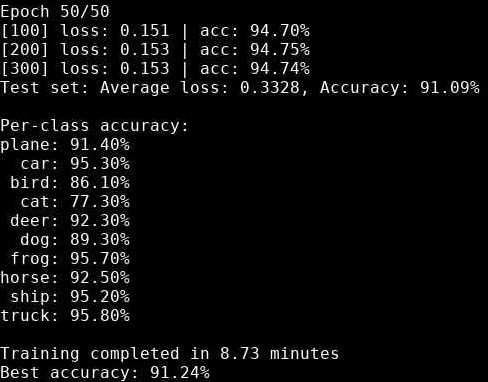
\includegraphics[width=0.9\textwidth]{media/1stAssignment/cnn_zero_epoch_50.png}
            \vspace{-0.4cm}
            \caption{Zero-centered}
        \end{figure}
        \vspace{-0.6cm}
        \center \tiny Mean: (0.5, 0.5, 0.5),
        \vspace{-0.3cm}
        \center \tiny Standard Deviation: (0.25, 0.25, 0.25)
    \end{column}
\end{columns}
\end{frame}

% Frame 17: Architecture modifications
\begin{frame}
    \frametitle{Architecture: CNN vs MLP}
    \begin{columns}
        \begin{column}{0.5\textwidth}
            \begin{figure}[t]
                \centering
                \vspace{-0.4cm}
                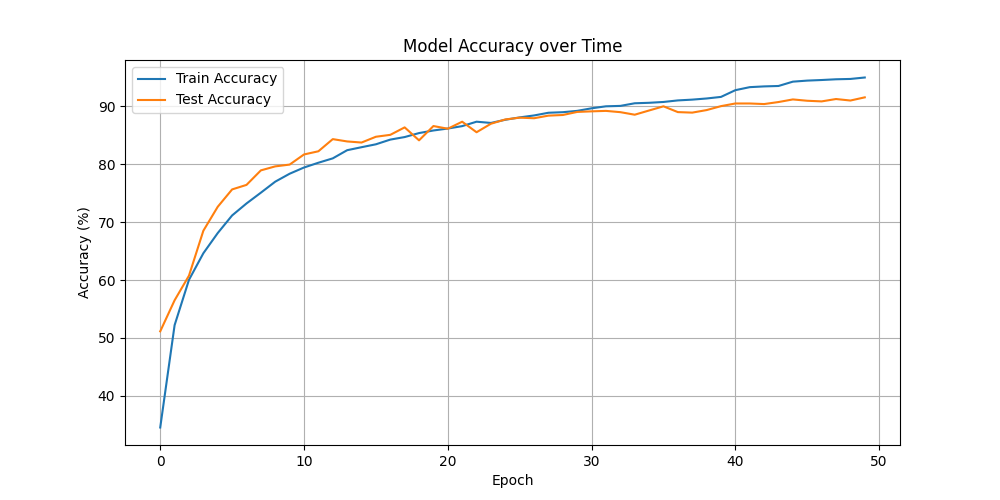
\includegraphics[width=0.9\textwidth]{media/1stAssignment/cifar10_cnn_accuracy.png}
            \end{figure}
            \vspace{-0.8cm}
            \begin{figure}[t]
                \centering
                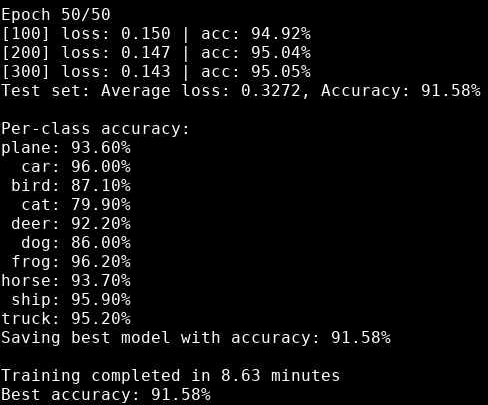
\includegraphics[width=0.9\textwidth]{media/1stAssignment/cnn_epoch_50.png}
                \vspace{-0.3cm}
                \caption{CNN: Last Epoch}
            \end{figure}
        \end{column}
    
        \begin{column}{0.5\textwidth}
            \begin{figure}[t]
                \centering
                \vspace{-0.4cm}
                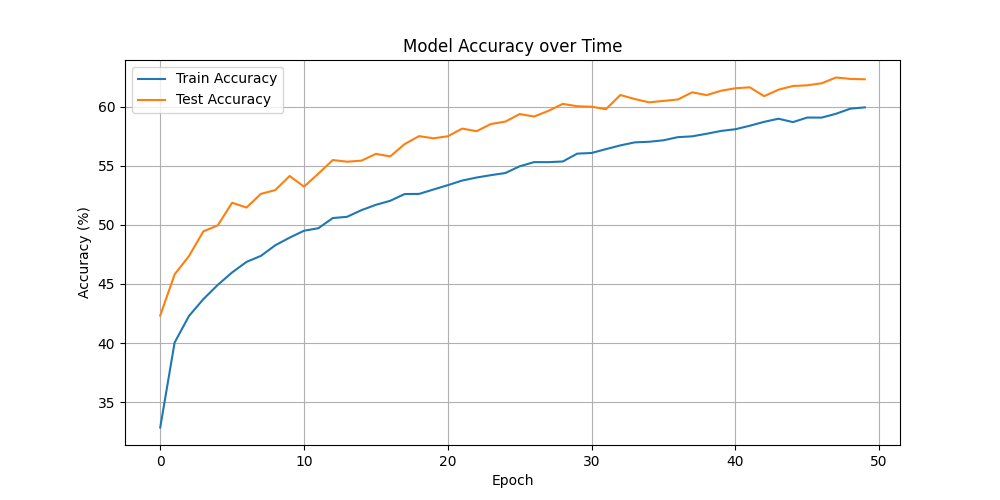
\includegraphics[width=0.9\textwidth]{media/1stAssignment/cifar10_mlp_accuracy.png}
            \end{figure}
            \vspace{-0.8cm}
            \begin{figure}[t]
                \centering
                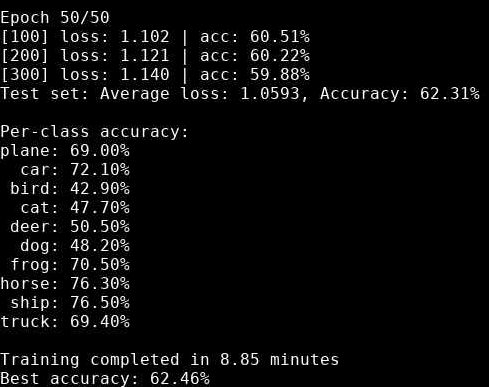
\includegraphics[width=0.9\textwidth]{media/1stAssignment/mlp_epoch_50.png}
                \vspace{-0.3cm}
                \caption{MLP: Last Epoch}
            \end{figure}
        \end{column}
    \end{columns}
\end{frame}

    
% Frame 18: True MLP Accuracy
\begin{frame}
\frametitle{True MLP Accuracy ft. Over-fitting and Transformations}
\begin{columns}
    \begin{column}{0.5\textwidth}
        The MLP model had the following architecture:
        \begin{itemize}
            \item Input Flatten Layer
            \item 3 Hidden fully-connected layers
            \item ReLU Activation Function
            \item Adam Optimizer
            \item 3 Dropout Layers 30\% 
            \item Normalization of each hidden layer
            \item Output Layer
        \end{itemize}
    \end{column}

    \begin{column}{0.5\textwidth}
        2 Important observations:
        \begin{itemize}
            \item Over-fitting isn't an issue, partly thanks to Dropout layers
            \item Transformations cause the model to generalize better but lead to 
            lower training accuracy
        \end{itemize}
    \end{column}
\end{columns}
\end{frame}

% Frame 19: MLP Demonstration
\begin{frame}
\frametitle{Demonstration}
\begin{figure}
    \centering
    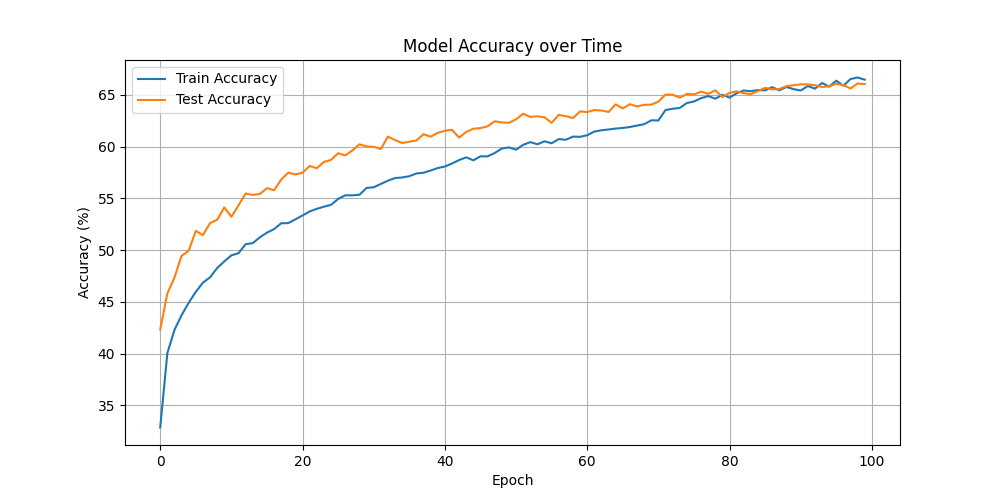
\includegraphics[width=1\textwidth]{media/1stAssignment/mlp_final_state.png}
    \caption{MLP: 100 Epochs}
\end{figure}
\end{frame}
